\sectionwithtoclink{The Heston Model}



\subsection{The Model}
The Heston model is defined by the following stochastic differential equations (SDEs)
\begin{align}
dS_t &= (r-q)\, S_t\,dt + \sqrt{v_t}\,S_t\,dW_t^{(1)}, \\
dv_t &= \kappa(\theta - v_t)\,dt + \sigma \sqrt{v_t}\,dW_t^{(2)} \\
\rho\,dt &= dW_t^{(1)} dW_t^{(2)}
\end{align}
where $r\geq 0$ is the constant risk-free rate, $q\geq0$ is a continuously paid dividend yield,
 $\kappa>0$ is the mean reversion factor,
 $\theta>0$ is the long-run variance,
 $\sigma>0$ is the so called vol-of-vol and
 $\rho\in[-1,1]$ is the correlation between the two Brownian motions driving the model,
 and $2\kappa\theta > \sigma^2$ which is called the Feller condition, forcing the variance process to be positive almost surely.




Applying It\^{o}'s lemma with $X_t=\log(S_t)$,
we get an equivalent model description
\begin{align}
dX_t &= \left(r -q- \frac{1}{2} v_t\right) dt + \sqrt{v_t}\, dW_t^{(1)}\\
dv_t &= \kappa(\theta - v_t)\,dt + \sigma \sqrt{v_t}\,dW_t^{(2)} \\
\rho\,dt &= dW_t^{(1)} dW_t^{(2)}
\end{align}
The neat thing about this extension is letting practitioners capture some of the behaviour they observe in real markets in their models,
namely letting the volatility process be stochastic and correlated with the underlying, also roughly letting the long-term vol converge towards
an expected level, matching the shape of the volatility surface flattening out on longer maturities. A complication with this model is the lack of an
analytical density for $X_T$, but knowing what we do about Fourier pricing we simply need the extended characteristic function to have an analytical expression,
which it turns out to do. But how does the model actually behave? To answer this question I've made some simulations using a Milstein-corrected Euler scheme as it is done
in~\cite{gatheral2006}

\begin{figure}[H]
  \centering
  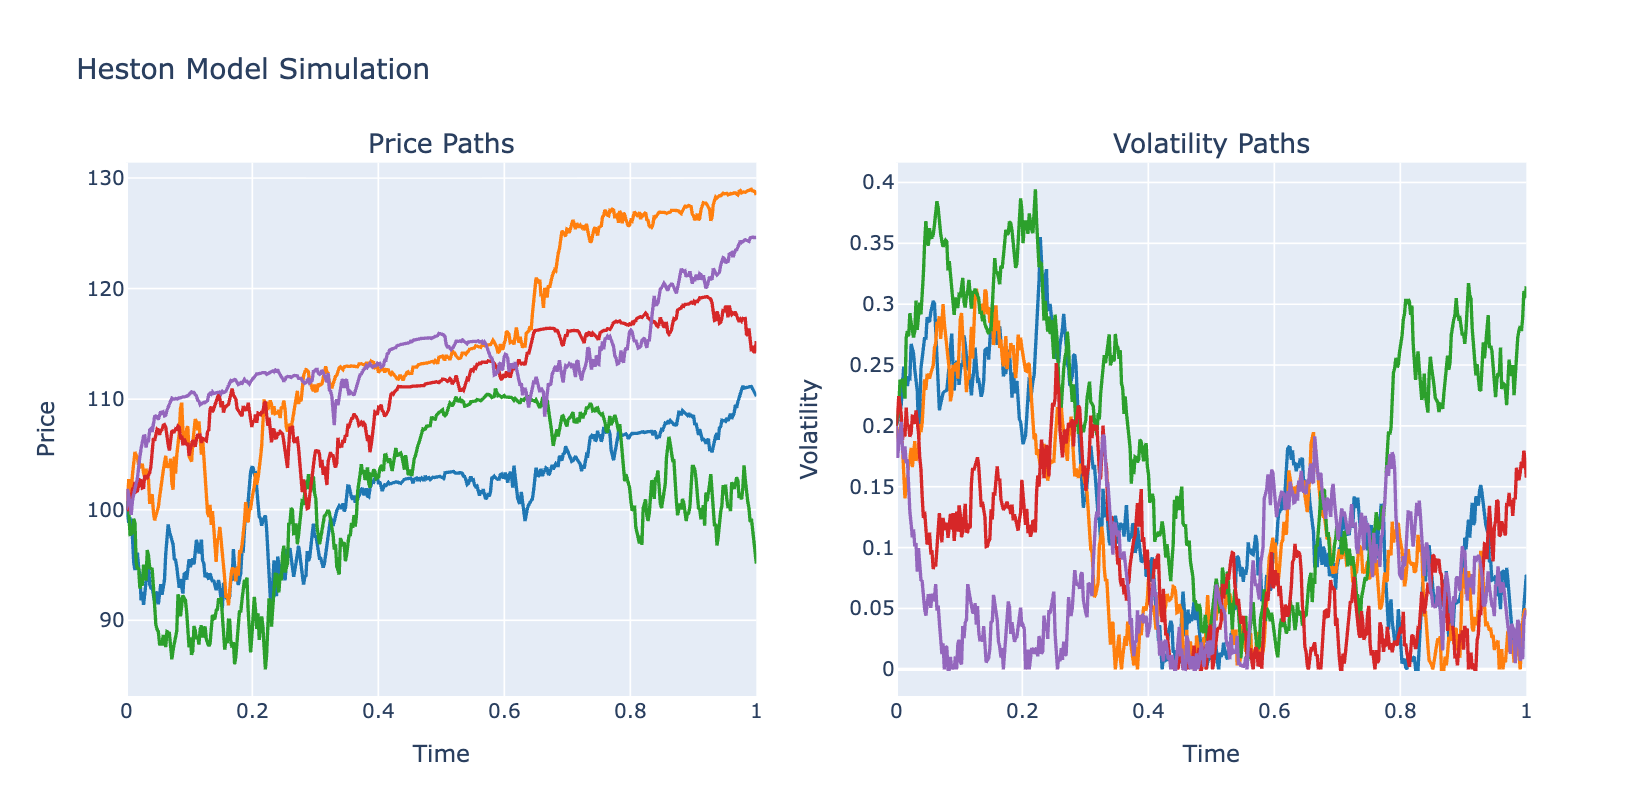
\includegraphics[width=\textwidth]{images/model_simulation.png}
  \caption{Simulated Heston model paths for the asset price and variance process using a Milstein-corrected Euler scheme ($S_0=100$, $v_0=0.04$, $\kappa=2.0$, $\theta=0.04$, $\sigma=0.6$, $\rho=-0.7$, $r=0.05$, $q=0.02$, $T=1$, $N=512$).}
  \label{fig:heston-simulation}
\end{figure}
In short, when markets go up they are more steady, but when they go down volatility spikes and we see more fluctuations.


\subsection{The Heston CF}
In this next part of the paper we will be deriving the characteristic function of the stochastic variable which solves the SDEs
which define the Heston model, we will be deriving the expression of the CF that Heston found in his original paper~\cite{heston1993},
starting from the Feynman--Kac conditions, which are essentially the same as what Heston does.
Assuming some regularity which the Heston SDEs satisfy, the Feynman--Kac formula gives us:
for every Borel function with polynomial growth f, a function $u:\mathbb{R}^+\times\mathbb{R}^n\rightarrow \mathbb{R}$ which satisfies
\begin{itemize}
\item[i)] $\frac{\partial u}{\partial t}(t, x) = Lu(t, x)\quad \forall t\geq0,x\in \mathbb{R}^n$\\
\item[ii)] $u(0, x) = f(x)\quad \forall x\in \mathbb{R}^n$\\
\item[iii)] $\exists C\in L^1_{loc}(\mathbb{R}),p\geq 0:\quad  \|\nabla u(t, x)\| \leq C(t)\left(1 + \|x\|^p\right)\quad \forall t\geq 0, x\in \mathbb{R}^n$,
\end{itemize}

satisfies
\begin{align}
\Rightarrow \mathbb{E}[f(X_t)] &=u(t,x)\quad\forall t\geq0,x\in \mathbb{R}^n
\end{align}

The idea of the proof is to use Feynman--Kac to get the characteristic function by setting $f(x,v)=e^{i\phi x}$ and guessing the solution
$u(t,x,v)$ for every $\phi\in\mathbb{R}$, and then extending it to the strip $\{b\in\mathbb{C}:\Im(b)\in[-1,0]\}$, thus getting the slightly extended characteristic function for the model.

\begin{theorem}[Heston Characteristic Function]
The characteristic function of $X_T = \log S_T$ under the Heston model is
\begin{equation}
\psi_T(\phi) = \exp\!\bigl(C(T,\phi) + D(T,\phi)\,v_0 + i\phi\,x_0\bigr), \quad \phi\in\mathbb{R},
\end{equation}
where $x_0 = \log S_0$. The auxiliary quantities are
\begin{align}
\xi &= \sigma\rho\,i\phi - \kappa, \\
d &= \sqrt{\xi^2 + \sigma^2(\phi^2+i\phi)}, \quad \Re(d)\geq 0,\\
g &= \frac{\xi-d}{\xi+d},\qquad D_1 = \frac{-\xi+d}{\sigma^2},
\end{align}
and the coefficient functions are
\begin{align}
D(T,\phi) &= D_1\,\frac{1-e^{dT}}{1-g\,e^{dT}}, \\[6pt]
C(T,\phi) &= (r-q)\,i\phi\,T
  + \kappa\theta\,D_1\!\left[T + \frac{1-g}{dg}
    \log\!\!\left(\frac{1-g\,e^{dT}}{1-g}\right)\right].
\end{align}
\end{theorem}

Let's start off by writing up the Feynman--Kac conditions within the model:

\begin{itemize}
\item[i)]
$\frac{\partial u}{\partial t} = \left(r-q-\frac{v}{2}\right)\frac{\partial u}{\partial x}
  +\kappa(\theta-v)\frac{\partial u}{\partial v}
  +\frac{v}{2}\!\left(\frac{\partial^2 u}{\partial x^2}+\sigma^2\frac{\partial^2 u}{\partial v^2}\right)
  +\sigma\rho v\frac{\partial^2 u}{\partial x\,\partial v}$
\item[ii)] $u(0, x, v) = \exp(i\phi x)$
\item[iii)] $\exists C\in L^1_{loc}(\mathbb{R}),p\geq 0:\quad  \|\nabla u(t, x, v)\| \leq C(t)\left(1 + \|(x,v)\|^p\right)\quad \forall t\geq 0, (x,v)\in \mathbb{R}^2$,
\end{itemize}
we make an affine ansatz
\begin{equation}u(t,x,v,\phi)= \exp(C(t,\phi)+D(t,\phi)v+i\phi x)\end{equation}
where we can calculate all the relevant partial derivatives
\begin{equation}
\begin{aligned}
u_x &= i\phi \,u, \\
u_v &= D\,u, \\
u_t &= (C' + D'v)\,u, \\
u_{xx} &= -\phi^2\,u, \\
u_{vv} &= D^2\,u, \\
u_{xv} &= i\phi D\,u.
\end{aligned}
\end{equation}
\begin{equation}i)\Leftrightarrow (C'+D'v)u= (r-q-\frac{1}{2}v)i\phi \,u+\kappa(\theta-v)D\,u+v\frac{1}{2}(-\phi^2\,u+\sigma^2 D^2\,u)+\sigma v\rho i\phi D\,u\end{equation}

We divide by $u$, which is non-zero (complex exponential), and combine like terms:
\begin{align}
C'+D'v = (r-q-\frac{1}{2}v)i\phi +\kappa(\theta-v)D+v\frac{1}{2}(-\phi^2+\sigma^2 D^2)+\sigma v\rho i\phi D\\
\Leftrightarrow C' + D'v=(r-q)i\phi + \kappa\theta D+v\left(-\frac{1}{2}i\phi-\kappa D+\frac{1}{2}(-\phi^2 + \sigma^2 D^2)+\sigma \rho\, i\phi D\right)
\end{align}
must be true for every v especially $v=0$ thus
\begin{align}
C' &=(r-q) i \phi+\kappa\theta D\\
D' &= \frac{1}{2}\sigma^2 D^2-\frac{1}{2}(\phi^2 + i\phi)+D(\sigma \rho\, i\phi -\kappa)
\end{align}
and similarly for ii) implies
\begin{equation}D(0)=0, \quad C(0)=0\end{equation}

The equation for $D$ is just an ODE, so let's solve it more specifically it is a Riccati equation of the form
\begin{equation}D'(t)=a(t)D(t)^2+b(t)D(t)+c(t)\end{equation}
with $a,b,c$ being constants in $t$, $f(t,D)= aD^2+bD+c \in C^\infty$ is locally Lipschitz in $D$ and a solution exists at least in some ball around $0$, which will be our $D$ from now on.\\
Let's start by finding the roots. First, define $\xi =\sigma \rho\, i\phi -\kappa$:
\begin{align}
0&= \frac{1}{2}\sigma^2 D^2-\frac{1}{2}(\phi^2 + i\phi)+D\xi\\
\Rightarrow D&=\frac{-\xi\pm d}{\sigma^2}
\end{align}
with $d=\sqrt{\xi^2+\sigma^2(\phi^2+i\phi)}$
thus by defining the roots we get
\begin{align}
D_1 &= \frac{-\xi+ d}{\sigma^2}\\
D_2 &=\frac{-\xi- d}{\sigma^2}\\
D'&=\frac{1}{2}\sigma^2(D-D_1)(D-D_2)
\end{align}
The solution to this ODE doesn't necessarily hit the roots, but we still need to note them so as not to divide by zero.\\
Here I should mention that if $0$ is a root then $D(t)=0$ solves the ODE, and by uniqueness must be the solution.

For now let's assume $D\neq D_1,D_2,\quad D_1\neq D_2,\quad D_1,D_2\neq 0$:
\begin{align}
\frac{1}{(D-D_1)(D-D_2)}&=\frac{1}{D_1-D_2}\left(\frac{1}{D-D_1}-\frac{1}{D-D_2}\right)
\end{align}
so for $D(t)\neq D_1,D_2$
\begin{align}
\frac{D'(t)}{(D(t)-D_1)(D(t)-D_2)}&=\frac{1}{D_1-D_2}\left(\frac{D'(t)}{D(t)-D_1}-\frac{D'(t)}{D(t)-D_2}\right)\\
\Rightarrow \frac{1}{2}\sigma^2&=\frac{1}{D_1-D_2}\left(\frac{D'(t)}{D(t)-D_1}-\frac{D'(t)}{D(t)-D_2}\right)
\end{align}
we remember that for u differentiable and $u(t)\neq 0$
\begin{equation}\frac{d}{dt}\log(u(t))=\frac{u'(t)}{u(t)}\end{equation}
by setting $u_1(t)=D(t)-D_1,\quad u_2(t)=D(t)-D_2$
\begin{align}
\frac{d}{dt}\log(D(t)-D_1\bigr) &=\frac{D'(t)}{D(t)-D_1}, \\
\frac{d}{dt}\log(D(t)-D_2\bigr) &=\frac{D'(t)}{D(t)-D_2}.\\
\Rightarrow\frac{d}{dt}\left[\frac{1}{D_1-D_2}\log\left(\frac{D(t)-D_1}{D(t)-D_2}\right)\right] &= \frac{1}{2}\sigma^2.\\
\Rightarrow\log\left(\frac{D(t)-D_1}{D(t)-D_2}\right)&=\frac{1}{2}\sigma^2(D_1-D_2)\,t + C\\
 D_1-D_2&=\frac{2d}{\sigma^2}\\
\Rightarrow\log\left(\frac{D(t)-D_1}{D(t)-D_2}\right)&=d t +C\\
\Leftrightarrow\frac{D(t)-D_1}{D(t)-D_2}&=\exp(dt+C)\\
\Leftrightarrow D(t)-D_1&=\exp(dt+C)(D(t)-D_2)\\
\Leftrightarrow D(t)(1-\exp(dt+C))&=D_1-D_2\exp(dt+C)\\
\Leftrightarrow D(t)&=\frac{D_1-D_2\exp(dt+C)}{1-\exp(dt+C)}
\end{align}
imposing the initial condition $D(0)=0$ and by renaming $\exp(C)=g$
\begin{align}
0=\frac{D_1-D_2g}{1-g}\Leftrightarrow g&=\dfrac{D_1}{D_2}=\frac{-\xi+d}{-\xi-d}=\frac{\xi-d}{\xi+d}\\
\Rightarrow D(t)&=D_1 \frac{1-\exp(dt)}{1-g\, \exp(dt)}
\end{align}

we should also consider if we ever have $D_1=D_2$
the short answer is no since:
\begin{align}D_1=D_2\Leftrightarrow d&=0\Leftrightarrow d^2=0\\
(\sigma \rho i \phi - \kappa)^2
&= \kappa^2 - 2\kappa \sigma \rho i \phi - \sigma^2 \rho^2 \phi^2\\
d^2&= \kappa^2 + \sigma^2(1-\rho^2)\phi^2 + i\phi(\sigma^2 - 2\kappa \sigma \rho)
\end{align}

but we assume  $\kappa>0,|\rho|\leq 1 \Rightarrow \Re (d^2)>0\Rightarrow d\neq 0$
thus we can never have $D_1=D_2$ but having a 0-root can and will happen actually
\begin{equation}D' \text{ has 0 as root}\Leftrightarrow \phi^2+i\phi=0\Leftrightarrow \phi\in \{0,-i\}\end{equation}
but $\phi\in \mathbb{R}$ thus
\begin{equation}\Leftrightarrow \phi=0\end{equation}
we've proven that when we have 2 non-zero roots that for  $D(t)\notin \{D_1,D_2\}$
\begin{equation}D(t)=D_1 \frac{1-\exp(dt)}{1-g\, \exp(dt)}\end{equation}
but does D ever hit the roots? i.e
\begin{equation}D_1,D_2\overset{?}{\in}D(\mathbb{R})\end{equation}
the answer is no. for $D_1$
\begin{align}
\frac{1-\exp(dt)}{1-g\, \exp(dt)}&= 1\\
\Leftrightarrow g&=1
\end{align}
this we have shown can never be the case under the Heston assumptions\\
$D_2$?
again no.
\begin{align}
D_2=&D_1 \frac{1-\exp(dt)}{1-g\, \exp(dt)}\\
\Leftrightarrow 1=g\frac{1-\exp(dt)}{1-g\, \exp(dt)}=&\frac{1-\exp(dt)}{g-\, \exp(dt)}\\
\Leftrightarrow g=&1
\end{align}
same argument, thus the function never hits the "roots"
we then have solutions for every $\phi\in\mathbb{R}$
\begin{equation}
D(t,\phi) =
\begin{cases}
0 & \text{if } \phi = 0 \\[4pt]
D_1 \dfrac{1-\exp(dt)}{1-g\,\exp(dt)} & \text{otherwise}
\end{cases}
\end{equation}
where $D_1=\dfrac{-\xi + d}{\sigma^2}$, $g=\dfrac{\xi-d}{\xi+d}$, $d=\sqrt{\xi^2+\sigma^2(\phi^2+i\phi)}$, $\xi =\sigma \rho\, i\phi -\kappa$.

So now it's time to find $C$.
This is a little easier since we simply have a functional expression.\\
In both cases we note that the functional expression $f(t,\tilde{c})=g(t)$ is continuous in $t$ and constant in $\tilde{c}$, making it Lipschitz in $\tilde{c}$ not just locally but globally.
\begin{align}
C' &=(r-q) i \phi+\kappa\theta D
\end{align}
we still need to split into 2 cases lets start with the easy one
for $\phi=0$
\begin{equation}C'(t)=0,\quad C(0)=0\Rightarrow C(t)=0\end{equation}
is a solution then by uniqueness the only one.\\
for $\phi\neq 0$
\begin{align}
C' &=(r-q) i \phi+\kappa\theta D_1 \frac{1-\exp(dt)}{1-g\, \exp(dt)}\\
\Rightarrow C(t)&=(r-q)i\phi t +\kappa \theta D_1\int_0^t{\frac{1-\exp(ds)}{1-g\, \exp(ds)}ds}
\end{align}
to evaluate the integral we guess and check with the ansatz, for some constant $A$,
\begin{align}
J(t)&=t+A\log\!\left(\frac{1-g\,\exp(dt)}{1-g}\right)\\
J'(t)&=1-A \, g \, d \frac{\exp(dt)}{1-g\,\, \exp(dt)}\\
&=\frac{1-g\,\exp(dt)-A\, d\, g\,\exp(dt)}{1-g\,\, \exp(dt)}
\end{align}
for $J'(t)=\frac{1-\exp(dt)}{1-g\,\exp(dt)}$ the numerator requires
\begin{align}
    1&=g+A\, d\, g\\
    \Leftrightarrow A\, d&=\frac{1}{g}-1\\
    \Leftrightarrow A&=\frac{1-g}{dg}
\end{align}
Small problem here: we want to use the complex version of the fundamental theorem of calculus.
To do that we need both the real and imaginary parts of $\log(1 - g\,\exp(dt))$ to be differentiable, for $\Re(d)<0$ and large $t$, it might not even be continuous,
as the argument might ``swirl'' around the origin and jump $2\pi i$. We fix this by choosing the complex root which has $\Re(d)> 0$, making $|g|<1$.
This fix does not fully solve the problem, as the argument breaks for large enough $T$'s. This instability of the original Heston CF is well
documented in The Little Heston Trap~\cite{albrecher2007}. An alternative and equivalent version of the Heston CF without this problem is documented by Germano et al.~\cite{germano2017} and del Ba\~{n}o Rollin~\cite{delBanoRollin2010}.
In Germano et al.~\cite{germano2017} they even show that we can find analytical gradients using similar Fourier methods as the ones covered here. That aside, picking a branch with $\Re(d)\geq 0$ works for small enough $t$'s.



By the fundamental theorem of calculus
\begin{equation}C(t)=(r-q) i \phi t +\kappa \theta D_1\left[ t+\frac{1-g}{dg}\log\left(\frac{1-g\,\exp(dt)}{1-g}\right)\right]\end{equation}
with
\begin{equation}C(0)=0+\kappa \theta D_1 (0+0)=0\end{equation}
and we are done. We now have functional forms for C,D such that
\begin{equation}\exp(C(t,\phi)+D(t,\phi)v+i\phi x) \text{ solves the PDE } \frac{\partial u }{\partial t}=Lu\end{equation}
and satisfies the boundary condition $u(0,x,v)=\exp(i\phi x)$\\

So the solution satisfies i)--ii). Now let's check iii). Remember that:
\begin{equation}u_x=i\phi u,\quad u_v=Du\end{equation}
then
\begin{align}
\|\nabla u(t,x,v)\|&\leq|u(t,x,v)|(|\phi|+|D(t)|)\\
&=(|\phi|+|D(t)|)\,\,\exp(\Re (C(t))+v\Re (D(t)))\\
&=C^*(t)
\end{align}
Everything is continuous, so $C^*$ is locally integrable:
\begin{equation}\|\nabla u(t,x,v)\| \leq C^*(t)(1+\|(x,v)\|^0)\end{equation}
so iii) holds with $p=0$. By this we can conclude that
\begin{equation}\psi(\phi)=\exp(C(t,\phi)+D(t,\phi)v+i\phi x)=\mathbb{E}[\exp(i\phi X_t^{(x,v)})]\end{equation}
for every fixed $\phi\in \mathbb{R}$
but this is exactly the definition of the characteristic function!

Now we need to extend it for the purpose of using the Lewis style formula for the prices that we found earlier, the extension is done in the paper Ba\~{n}o Rollin et al.~\cite{delBanoRollin2010}.
In the paper they show that the CF extends to and is analytic on $[-1,0]$ via an equivalent expression of the moment generating function and thus the CF, then using an analytical continuation argument.





just to end this off we need to make sure that $\psi(\cdot -i/2)\in L^1$. For $u\in\mathbb{R}$ and $\phi=u-i/2$, the term $i\phi x_0=(iu+\tfrac{1}{2})x_0$ contributes $\tfrac{x_0}{2}$ to the real part (the $ix_0 u$ piece is purely imaginary), so the original Heston CF gives
\begin{align}
  |\psi(u-i/2)|
  &=\exp\!\Bigl(\tfrac{x_0}{2}+\Re\bigl(C(T,\,u-i/2)\bigr)+v_0\,\Re\bigl(D(T,\,u-i/2)\bigr)\Bigr)\\
  &\leq K\cdot\exp(-\gamma|u|)\quad\forall u\in\mathbb{R}\\
  &\Rightarrow \psi(\cdot-i/2)\in L^1
\end{align}
the expressions for $\gamma,K$ are noted in the appendix\\
We've now found an expression for the extended CF of $X_T$ on the strip $\{z\in \mathbb{C}:\Im(z)\in(-1,0]\}$ and shown that $\{z\in \mathbb{C}:\Im(z)=-\frac{1}{2}\}\subseteq \mathcal{S}_{-\psi}$,
which also implies that the log spot dynamics are actually absolutely continuous, but more importantly for this paper, that we have an expression for the Heston CF which satisfies the conditions
necessary to use the Lewis style pricing formula that we've derived earlier.



